\documentclass{article}
\usepackage{graphicx, hyperref}

\title{RNGeo Field Guide: end-to-end development with Ren \textbf{(WORK IN PROGRESS)}}
\author{Li Xuan Tan}
\date{\today}

\begin{document}

\maketitle

\section{Inspiration}

\begin{center}
    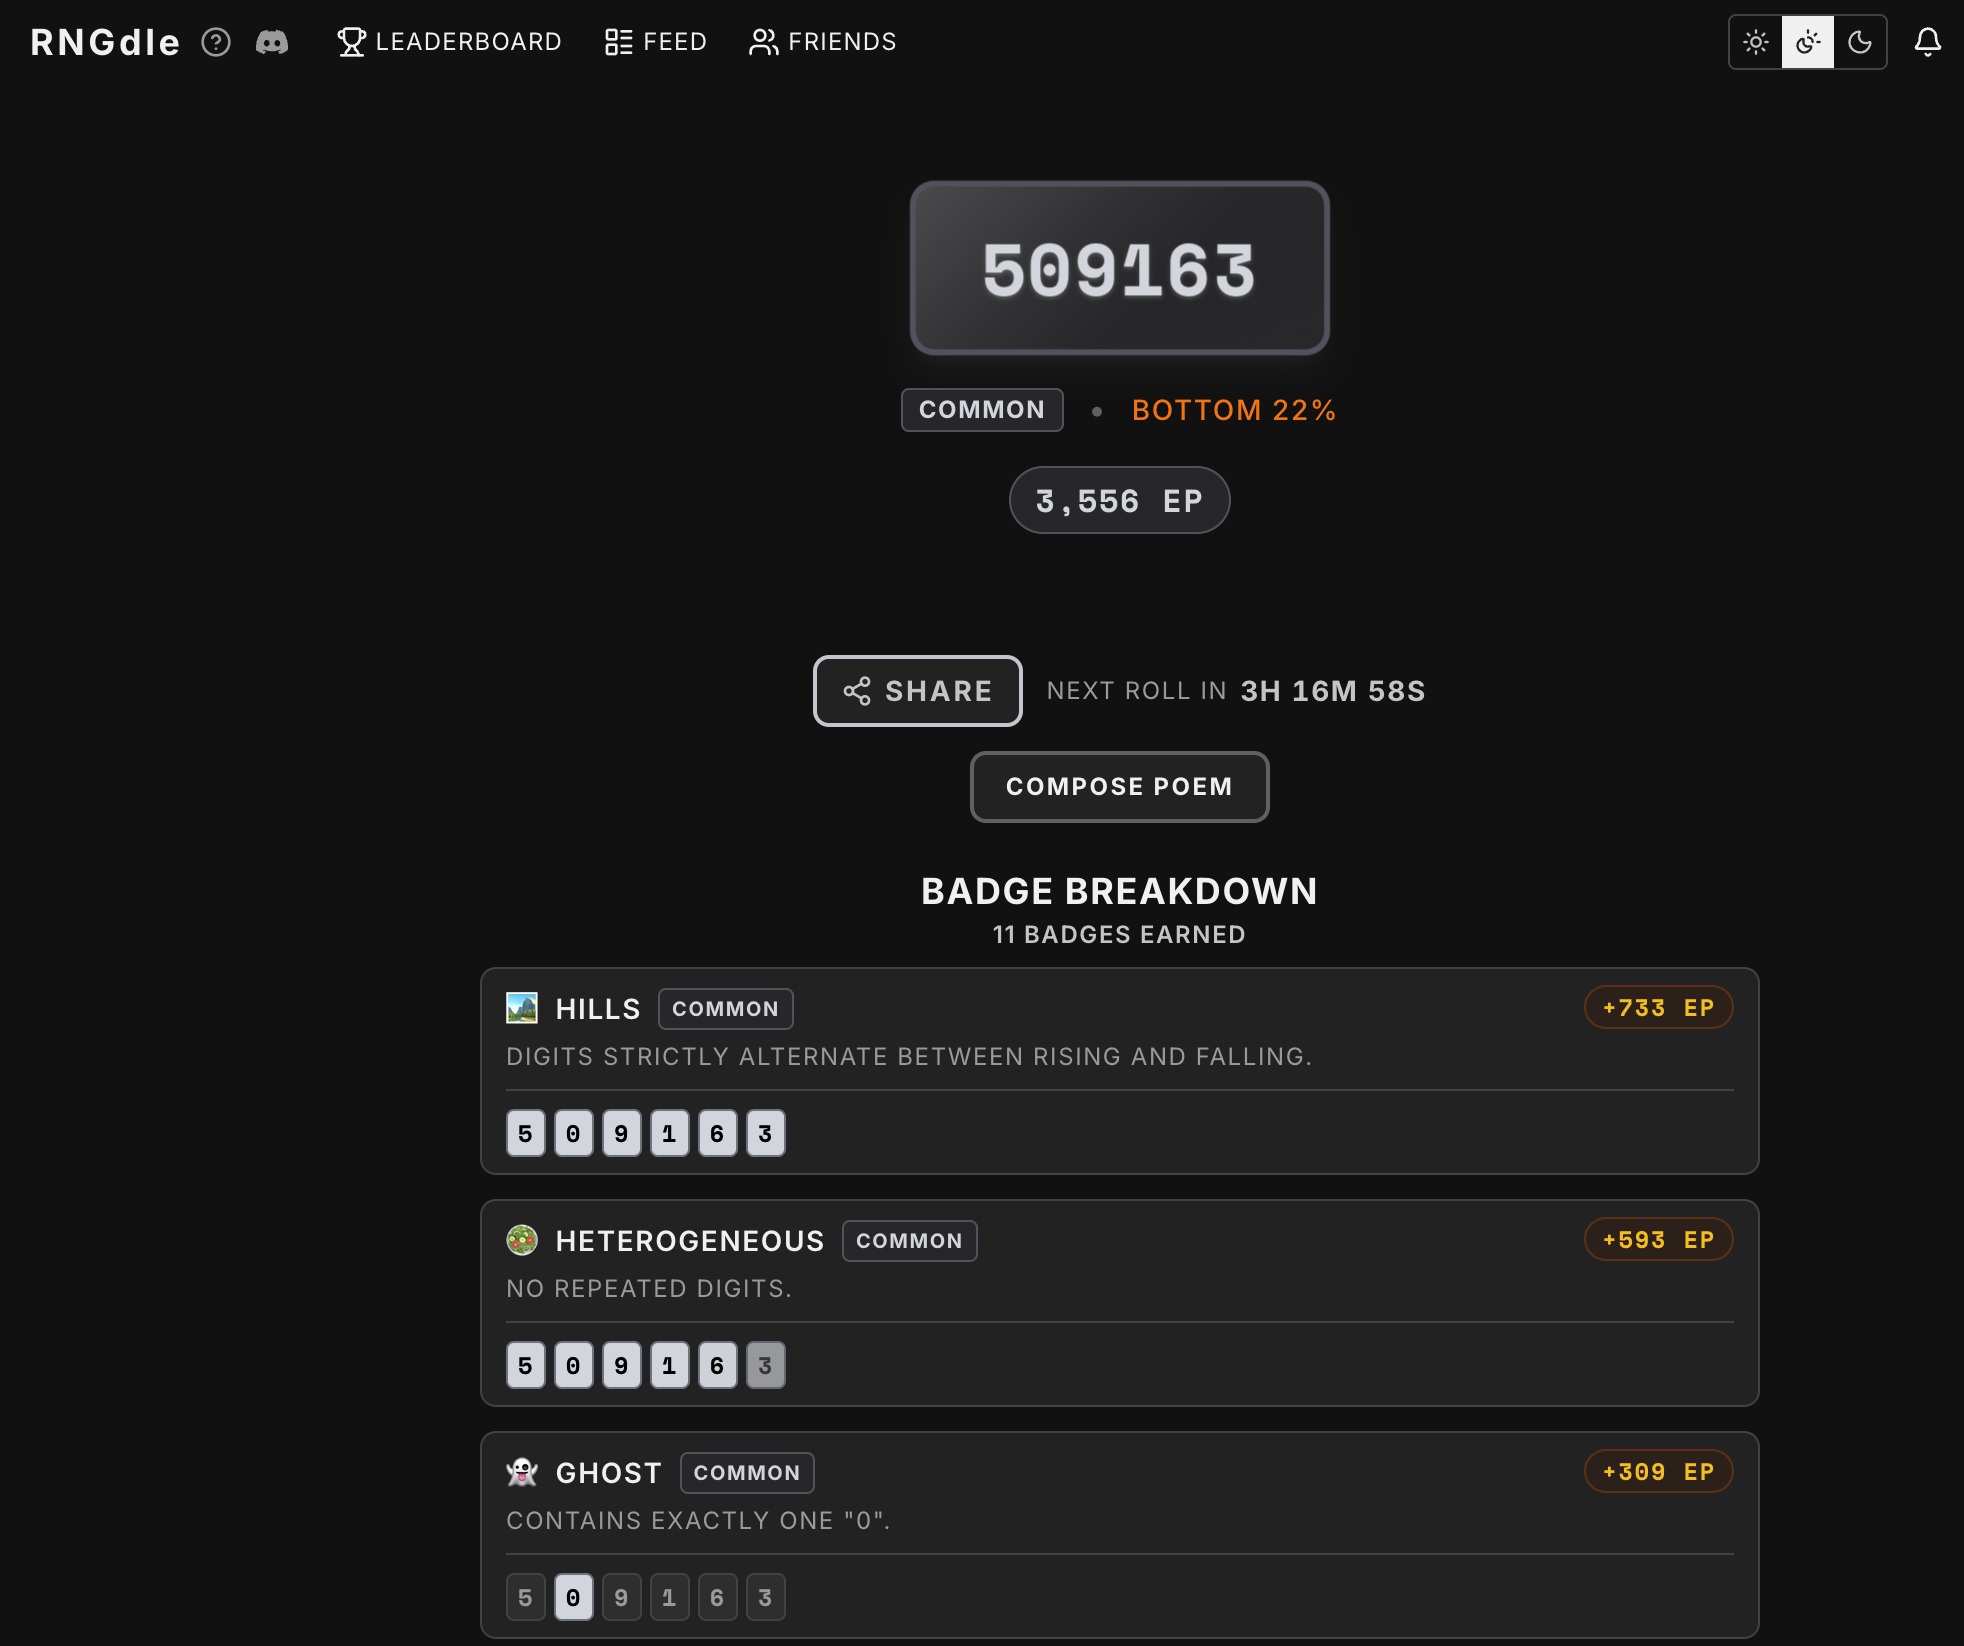
\includegraphics[width=0.9\textwidth]{media/Screenshot 2026-07-09 at 13.43.01.png}
    
    Figure 1: Interface of RNGdle.
\end{center}

Inspired by a combination of Foursquare and RNGdle.

\section{Architectural overview}

\subsection{Client}
Client imports its keys and a pre-registered name/UUID combo from the keygen script.
It periodically samples location (32 bits each lat/long, scaled by 1e5 and rounded to nearest integer) and timestamp (64 bits Unix seconds), encodes these three integers into the first 128 bits of a ciphertext, then encrypts and sends the result to the server using the \verb|get_score| API.

When the server responds, the client decrypts and decodes the result as follows:
\begin{itemize}
    \item slot 0 holds the "PRF score", a pseudorandom score in $[0, 2^{20})$ seeded by the location/timestamp data;
    \item slots 1 through 64 hold the "POI scores", a Gaussian score for each POI in $[0, \approx 2^{20})$ that peaks when the encrypted location is directly on the POI and falls off exponentially with stdev $\sigma \approx 250m$.
    \item slots 65+ hold the "POI tag", a single bit which indicates whether the encrypted location is within $d \approx 100m$ of a POI, followed by the ASCII-into-binary-encoded name of the POI if nearby.
    \item the last 256 slots hold the result of the encrypted PRF for client-side verification.
\end{itemize}

\subsection{Server}
The webserver exposes the following APIs:
\begin{itemize}
    \item \verb|init_user| takes in a display name and public context, returning a UUID which is associated with a Session object containing this context. Sessions can be evicted to a database following LRU. 
    \item \verb|get_score| takes in a ciphertext in the client's format and performs three branches of computations: the PRF score, the POI score (fold binary location back into decimal, use equirectangular formula to approximate POI distance, then approximate the Gaussian score via repeated squaring. Gaussian computation can be batched by placing all the POI distances in slots 1-64), and the POI tag (fold and approximate distance, then apply encrypted-sign function to determine if this distance is less than $d$).
    \item \verb|submit_score| receives a score (plaintext) and a UUID, maintaining a leaderboard with the top 20 submissions from unique users each day, resetting at 6pm PT. \verb|get_leaderboard| allows clients to query this leaderboard and display it locally.
\end{itemize}

\subsection{Keygen}
Keygen script runs on a laptop, taking a display name and registering it with the server's \verb|init_user| API, then receiving a UUID back.

Keys are generated on CPU, then the public context is serialized and uploaded to server over the internet. 
User is given a .txt file containing the serialized private key, which should only be transferred P2P to the client device and never shared elsewhere.

\vspace{1cm}

The following sections describe (roughly in chronological order) some of the major problems we encountered in developing RNGeo, and what solutions or workarounds we took.

\section{Mobile libraries}

\noindent\fbox{%
    \begin{minipage}{\textwidth}

    \textbf{Problem:} Ren doesn't have native support for mobile backends, only CUDA and Python's CPU fallback (for which runtimes don't exist/aren't efficient on iOS/Android).

    \end{minipage}%
}
\vspace{0.3cm}

\textit{Solution process:} Reimplement critical functions (encode/decode) in Swift and Kotlin - see rngeo codebase, offload keygen to a desktop helper script which is necessary anyway due to heavy compute requirement ($\approx$15 min on laptop CPU, 5 sec on apollo GPUs).

From the desktop script, transfer only the necessary private key to mobile app by serializing to a .txt file (4MB on toy params), while the public context is uploaded to server and indexed by UUID.

(Note from prototypes track discussion: there are plans for future client libraries once appropriately specced-out)

\section{Ren's context model}

\noindent\fbox{%
    \begin{minipage}{\textwidth}

    \textbf{Problem:} Since Ren works using enabled contexts that provide the necessary keys for any operation, how do we enforce the server/client key separation? 
    Server must hold all the evaluation keys (and the public key) but never the secret key, whereas the client must hold the private key but doesn't need others.

    Relatedly, how do we pass contexts between eg. server and client?

    \end{minipage}%
}
\vspace{0.3cm}

\textit{Solution process:} Serialize contexts using Ren's builtins (which also allow serializing only public context), then pass that data over HTTP sockets.
Contexts are generally not passed to modules, with only the server in \verb|app.py| opening contexts before calling functions that require keys.

\section{Computing a PRF}

\noindent\fbox{%
    \begin{minipage}{\textwidth}

    \textbf{Problem:} How do we compute a pseudorandom function (PRF) given a seed encrypted under CKKS?

    \end{minipage}%
}
\vspace{0.3cm}

\textit{Solution process:} First step is to choose a suitable PRF that is FHE-friendly. 
Initial thought was ChaCha20 as it involves mostly adds/XORs/rotations, but turns out this circuit is actually pretty deep when implemented. 
The next attempt was a substitution-permutation network (SPN) using a simple low-degree polynomial for the S-box, but this did not provide enough mixing - ideally, a single bit flip in the input would flip around half of the output bits in a PRF.

\href{https://eprint.iacr.org/2020/1335.pdf}{HERA} is another HE-friendly stream cipher that is designed to be high-performance, but needs general reduction mod $p$ which is not available (?).
Settled on \href{https://eprint.iacr.org/2018/181.pdf}{Rasta}, a cipher on binary inputs (which we already use to encode location/timestamp) using relatively low depth.

The final PRF uses a secret environment variable (server-side) and the current leaderboard window to seed the Rasta round constants, then takes as input the encrypted (location, timestamp) data encoded in binary.

\section{Precision limits}

\noindent\fbox{%
    \begin{minipage}{\textwidth}

    \textbf{Problem:} $\log(QP) \leq 1747$ for secure params, and the circuit requires $\approx$ 34 levels, so \texttt{log\_precision} $\leq 44$ is required.

    \end{minipage}%
}
\vspace{0.3cm}

\textit{Solution process:} Bound the play area to a $\approx 1 \deg$ square to allow for more precise local gameplay (error grows quadratically with relative size of the play box, in terms of the desired $\sigma$).
Since the location is already encoded in binary, it's fairly simple to check that the first $k$ bits match the play box for some $k$ ($k=15$ prefix gives $\approx 1.3 \deg$ square box), but we also wanted to center the gameplay around the office in FiDi which the larger grid wouldn't allow.

The solution was to make the gameplay box be a 3x3 grid of $k=17$ boxes, which works pretty well both for size and centering.
This is actually depth-free because we can just sum the 9 disjoint indicator branches.

\section{To bootstrap, or not to bootstrap}

\noindent\fbox{%
    \begin{minipage}{\textwidth}

    \textbf{Problem:} Low precision (previous issue) causes large errors to accumulate. Can we use high-precision bootstrapping to allow for higher-precision, lower-depth params?

    \end{minipage}%
}
\vspace{0.3cm}

\textit{Solution process:} Key size explodes - we measured up to 50 GB VRAM in use per-user at high-precision bootstrapping params, so this was shelved temporarily. 

\section{Edge (aka Cloudflare) limitations}

\noindent\fbox{%
    \begin{minipage}{\textwidth}

    \textbf{Problem:} JIT capture/replay becomes really important to keep runtime down as complexity and user load grows. 
    However, the initial capture took up to 250 seconds at one point in development, exceeding the Cloudflare limit of 100 seconds per synchronous request.

    \end{minipage}%
}
\vspace{0.3cm}

\textit{Solution process:} Trim nodes in the evaluation graph by combining/batching inputs to some of the computations (eg. the Gaussian scoring and the encrypted-sign tagging). 
Registering some of the non-power-of-2 rotation keys that were used by eg. the Rasta PRF also helped since Ren no longer had to BFS-compose long chains of rotations.

\section{Key sizes}

\noindent\fbox{%
    \begin{minipage}{\textwidth}

    \textbf{Problem:} Key sizes are $\approx$ 0.9 GB under toy params and $\approx$ 20 GB under secure. 
    Large keys cause slow keygen and upload, high VRAM pressure, inability to retain contexts in memory requires frequent cache accesses.

    \end{minipage}%
}
\vspace{0.3cm}

\textit{Solution process:} Trimming rotation keys gave about a 25\% reduction in our case, but this effectiveness will largely depend on what keys are actually being used and whether the BFS-composition costs more in runtime/graph complexity.

Seeded keys have been implemented; the pseudorandom public part $a$ of the ciphertext $(a, b)$ is now sent as a 48-byte seed, basically halving the upload.
To use this, you must verify that the PRF (generating $a$, not the scoring PRF) behaves identically across machines given the same seed.
Server-side recovery from seed took $\approx$15 sec on Apollo at secure params, and $\approx$15 GB keys per user remain resident in VRAM so we still have to use a pretty aggressive LRU policy.

\section{Slow Python fallback}

\noindent\fbox{%
    \begin{minipage}{\textwidth}

    \textbf{Problem:} Keygen at secure params took 2.5 hours to fully realize all polys when run on the CPU backend; however, we need to run keygen on non-CUDA devices for the demo, as having the keygen on-server breaks the security assumption.

    \end{minipage}%
}
\vspace{0.3cm}

\textit{Solution process:} Swift implementation of seeded keygen brought the time down to 5.5 min on M4 series MacBook Pro/Mac mini. Andrii is working on a Rust implementation for better cross-platform support.

\section{Using the DGX Spark}

\noindent\fbox{%
    \begin{minipage}{\textwidth}

    \textbf{Problem:} TBD

    \end{minipage}%
}
\vspace{0.3cm}

\textit{Solution process:} TBD

\end{document}